
\begin{abstract}
Design equations are a required tool in the  analog designers
toolbox. In this paper we show how one can calculate the required
parameters for 
comparator-based switched-capacitor circuits for use in a pipelined ADC. The parameters are
capacitance ($C$), current ($I_0$), comparator delay ($T_d$), current
source output resistance ($R_o$) and comparator threshold 
($V_{ct}$). The design equations
are verified with behavioral simulations in SPICE and MATLAB.
\end{abstract}


%\keywords{
%\paragraph{Keywords}
\begin{keywords}
 Comparator-based switched-capacitor circuits, design equations,
 pipelined analog-to-digital converters
\end{keywords}
%}
\section{Introduction}
\IEEEPARstart{D}{ownscaling} of CMOS technology continue to challenge the analog
designer. Reduced power supply, due to reliability concerns
\cite{iwai99}, and reduced
transistor output resistance, due to shorter channels
\cite{annema05}, lead to low headroom and low intrinsic
gain. As a consequence, high DC gain
operational amplifiers (opamp) | the key component in most
switched-capacitor circuits | is hard to design in nano-scale
technologies. 

Techniques like correlated level shifting
\cite{gregoire08}, open-loop residue amplifiers \cite{murmann03}, gain calibration \cite{hernes07},  and
comparator-based switched-capacitor circuits (CBSC)  \cite{sepke06} have been
developed to solve  some of the challenges. The techniques either reduce the
gain requirements for a given resolution, or replace the
opamp completely. 


Introduced in
\cite{sepke06} CBSC is a completely new approach to switched-capacitor
circuits. It replaces the opamp with a comparator and a current
source. To demonstrate the technique a prototype 10-bit 8-MS/s 
2.5-mW pipelined ADC was presented at ISSCC 2006  \cite{sepke06}. The implementation was detailed in
\cite{fiorenza06}.
%A
%year later a 200-MS/s 8-bit 8.5-mW Zero-Crossing-Based pipelined ADC,
%which replaced the comparator with a zero-crossing detector,
%was presented \cite{brooks07}. These implementations were
%explained in more detail in
%\cite{fiorenza06} and \cite{brooks07a}. 

In this paper we discuss how to design CBSC circuits for
analog-to-digital converters. 

Before one starts simulating transistors in SPICE it is of utmost
importance to have a clear idea of the dominating error sources, and
how they should be handled. In that respect, tools like design
equations, mathematical simulations and behavioral SPICE simulations
are invaluable tools for the analog designer.

\paragraph{Design Equations}
 Based on the specification (how fast, how accurate, how
    little power) the parameters for different circuit blocks can be
    calculated. The design equations result in a place to start, a set of
    initial parameters to work with. 
\paragraph{Mathematics based simulation}
 Behavioral
  simulation in a mathematics based tool, like MATLAB or
  OCTAVE, is more complex than design equations, but more
  accurate. But it is still fast and a designer can sweep parameters
  to find optimal solutions.
\paragraph{SPICE simulation}
Behavioral level description in SPICE allow the designer to have a
top-level description of the circuit, with all circuit blocks defined.   
The functionality of circuit blocks is checked before circuit blocks
 are implemented with transistors. 

This paper is organized as follows: Section \ref{cdessc:opamp} review opamp based
switched-capacitor circuits. Section \ref{cdessc:cbsc} explain
comparator-based switched-capacitor circuits. A model of the output
voltage of a CBSC amplifier with a gain of two is described in Section
\ref{cdessc:outmod}. In Section \ref{cdessc:design}
we introduce a design methodology for CBSC circuits and show a design
example in Section \ref{cdessc:example}. Results of
simulations in MATLAB and SPICE verify our design equations in Section \ref{cdessc:sims}.


%-------------------------------------------------------
\section{Opamp based switched-capacitor circuits} \label{cdessc:opamp}
%-------------------------------------------------------
%switched-capacitor circuits are prevalent in  ADCs
%because of their robustness and accuracy. Doing
%arithmetic operations like summation, subtraction, multiplication 
%and division is possible in SC circuit with high accuracy. The
%accuracy of SC circuits is limited by capacitor matching, which can be
%accurately set in integrated circuits (on the order of 0.1 percent \cite{johnsmartin}).  

Switched-capacitor (SC) circuits are usually designed with an opamp feedback loop as shown in
Fig. \ref{cdesfig:sccmult}. Most SC circuits have two clock phases,
sampling and charge transfer. Fig. \ref{cdesfig:sccmult} is a  
amplifier where the input is sampled in phase $p_1$, and charge is
transferred from
$C_1$ to $C_2$ in $p_2$ by forcing $V_x$ to
ground. If the opamp has infinite gain the discrete time transfer
function for Fig. \ref{cdesfig:sccmult} is a  delayed
amplification, where the gain is determined by the capacitance
ratio.
\eqn{
H_0(z) = \frac{C_1+C_2}{C_2} z^{-1}
}
With finite gain in the opamp the transfer function is
\eqn{
H_1(z) = H_0(z) \times\frac{1}{1+(C_1/C_2+1)/A}
}
where $A$ is the DC gain of the opamp.  Finite gain in the
opamp reduce the gain of the SC amplifier.  For the remainder of this work we assume $C_1 = C_2$, so the
amplifier has a gain of two.

%Normally a gain error is not a significant problem, but in pipelined
%ADC a gain error cause static non-linearities, which 
%reduce the resolution.  In older technologies---
%like 0.18$\mu$m and 0.35$\mu$m --- a high DC gain requirement pose
%few problems. It is trivial to make two
%stage amplifiers with enough gain for high accuracy systems. And if a
%two-stage amplifier does not have enough gain, an opamp with cascoding, or gain boosting will. As the
%CMOS technology scales, however, it is increasingly
%difficult to achieve a high DC gain, mainly due to
%the decreased output resistance of nano-scale transistors. Speed can be
%traded against gain by increasing channel
%lengths, but this often an undesirable trade-of. 

\begin{figure}[htbp]
\centerline{ \includegraphics[width=\myfigwidth]{graphics/sccmult}}
  \caption{Switched-capacitor amplifier using an operational amplifier}
  \label{cdesfig:sccmult}
\end{figure}

\section{Comparator-based switched-capacitor circuit}\label{cdessc:cbsc}
It does not matter how a SC circuit arrive at the output
voltage. What matters is that the output voltage is correct when the 
next stage samples, which usually is at the end of charge transfer. 

Instead of an opamp a current source and a comparator can
be used \cite{sepke06}. An opamp forces the virtual ground condition
while CBSC charge the output with a current source and detect when
virtual ground is reached.

 An example of a single ended CBSC is shown in
Fig. \ref{cdesfig:sc-cbsc}, only charge transfer phase is shown, sampling
phase is equivalent to opamp based SC. 

At the start of charge transfer the output is reset to
the lowest voltage in the system (usually the negative supply
voltage), which ensure that $V_x$ start 
below the virtual ground (common mode). The current source is turned
on at the start of
reset and use reset to settle. When reset ends the current
source charge the output capacitance. The voltage at 
$V_o$ and $V_x$ rise until the comparator detects virtual ground ($V_x
 = V_{CM}=0$). Due to the comparator delay it takes a moment for the
 current source to turn off, which result in an overshoot. 

The
 overshoot can be corrected in several ways. One way is using two
 ramps \cite{sepke06}, one fast and
 one slow, the fast ramp does an estimate of the output voltage, while
 a slow ramp in the opposite direction discharge the 
 overshoot. Another is to change the threshold of the
 comparator to compensate for the overshoot \cite{brooks07a}.

%A
% fundamental difference between opamp based SC and CBSC is that Opamp based SC settle during charge
%transfer, CBSC never settle. The current from the current source is
%fully on until it is turned off, in an opamp based SC all currents in
%capacitors and switches (outside of the opamp) go asymptotically to
%zero as the opamp settles. In CBSC the current in capacitors and
%switches are in one of two states, constant or zero, and they are
%only zero when the final value has been determined. As a result, switch resistance cause offset and a
%non-linearity (switches have signal dependent resistance) \cite{fiorenza06}, \cite{brooks07a}. But effects
%can be minimized by splitting the current source \cite{brooks07a}, or
%reducing switch resistance. Reduced current helps, but the current
%in CBSC is
%proportional to frequency so high speed require high current.
%Our CBSC sample the output at the end of charge transfer, where as
%\cite{sepke06} and \cite{brooks07} sample when the current sources
%turn off. 

%The noise properties of
%comparator-based and zero-crossing-based converters has been
%exhaustively covered by \cite{sepke06th} and \cite{chow07} and
%will not be discussed in this work. 

A analytical model of the output voltage is
presented in the next section.

\begin{figure}[htbp]
\centerline{ 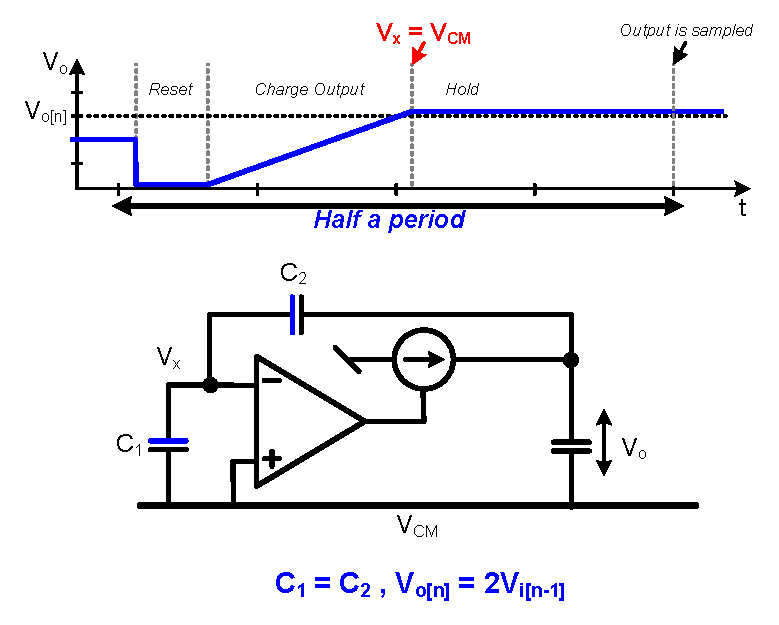
\includegraphics[width=\myfigwidth]{graphics/sc-cbsc}}
  \caption{Comparator-based switched-capacitor circuit}
  \label{cdesfig:sc-cbsc}
\end{figure}


\section{Model of CBSC output voltage}\label{cdessc:outmod}
%Modeling is important: equation based
%simulation tools, like MATLAB,  run behavioral level models in
%seconds, compared to minutes for behavioral level models in SPICE and
%days for a full pipelined ADC at transistor level. 

Assume finite resistance in current source. Kirchhoff's current law give the
differential equation
\eqn{
  I_0 = C_o \frac{d V_o(t)}{dt}  + V_o(t)/R_o
}
where $C_o$ is the capacitance at the output, $V_o$ is the
 output voltage, $I_0$ is the current in the current source and
$R_o$ is the output resistance of the current source. Solving the
differential equation yields.
\eqn{
\label{cdeseq:voout}
  V_o(t) = I_0 R_o \left (1 - e^{-\dfrac{t}{R_o C_o}} \right)
}
The time $t$ is the sum of $T_{V_I}$ | the time to charge to the ideal
output voltage ($V_o(t) = 2V_I$) | and the comparator delay
$T_d$. The ideal charge time $T_{V_I}$ is given by
\eqn{
  T_{V_I} =-ln \left(\frac{-2V_I}{R_o I_0}+1 \right) C_o R_o
} 
To compensate for the comparator delay the comparator threshold
($V_{ct}$) can be changed, so
the comparator start switching before $V_o = 2V_I$ is reached. Accordingly,
the charge time can be written as
\eqn{
\label{cdeseq:votime}
  t = -ln\left(-2\frac{V_I-V_{ct}}{R_o I_0}+1\right) C_o R_o + T_d
}
Inserting \req{votime} in \req{voout} results in
\eqn{
\label{cdeseq:vooutfin}
  V_o(t) = 2 e^{-\dfrac{T_d}{R_o C_o}}V_I + I_0R_o[1 - e^{-\dfrac{T_d}{R_o
      C_o}}(1 + 2\dfrac{ V_{ct}}{I_0R_o})]
}
The gain in of the amplifier should be two, but from \req{vooutfin} we
see the gain is smaller than two ($2e^{-T_d/R_oC_o}$).

 This gain error will cause
static non-linearities when a CBSC circuit is used in a pipelined
ADC. The gain error is a function of the comparator delay, the output
resistance and output capacitance. 
The last term in \req{vooutfin} is the
overshoot. 

In the next section we will use these equations to calculate the
necessary parameters for a CBSC circuit.

\section{CBSC design equations}\label{cdessc:design}
The SC circuit in Fig. \ref{cdesfig:sc-cbsc} finds use in pipelined ADCs
in the multiplying digital-to-analog converter (MDAC)
\cite{andersen05}. The necessary parameters for CBSC are capacitance
(C), current source current ($I_0$), comparator delay ($T_d$), current
source output resistance ($R_o$), and comparator threshold 
($V_{ct}$).

The first thing we need to calculate is the necessary sampling
capacitance given by \cite{wulff07}
\eqn{
\label{cdeseq:cap}
C = a_1 \times \dfrac{48 k T 2^{2B}}{V_{PP}^2} 
}
where $a_1$ is a constant larger than one, $k$ is Boltzmann's constant, $T$ is the
temperature in Kelvin, $B$ is the number of bits, and $V_{PP}$ is the
differential peak-to-peak signal swing. 

To estimate the required current we assume that the output ramp is
constant so
\eqn{
  V_o = \dfrac{I_0}{C_o} t
}
The current in the current source is then calculated from
\eqn{
\label{cdeseq:reqc}
  I_0 = \dfrac{C_o(V_{pp}/4 + V_{cm})}{\dfrac{1}{2f_s} - T_r}
}
where $V_{cm}$ is the common mode voltage, $f_s$ is the sampling
frequency, $T_r$ is the reset time and $C_o$ is the output capacitance
given by
\eqn{
  C_o = \dfrac{C_1C_2}{C_1+C_2}+C_L
}
where $C_1 = C_2 = C/2$, and $C_L$ is the capacitance of the next
stage. 

The comparator delay is chosen based on technology and noise
properties \cite{fiorenza06}.

The required output resistance of the current source is determined by
the gain error from \req{vooutfin}
\eqn{
\label{cdeseq:gainerr}
  1 -\epsilon_g = e^{-T_d/R_oC_o}
}
where $\epsilon_g$ is the gain error.  The required output resistance
is then
\eqn{
\label{cdeseq:reqro}
R_o = \dfrac{-T_d}{ln(1-\epsilon_g)C_o}
}

The comparator threshold ($V_{ct}$) compensate for the overshoot from
\req{vooutfin} given by
\eqn{
V_{off}  = I_0R_o \left[1 - e^{-\dfrac{T_d}{R_o
      C_o}}\left(1 + 2\dfrac{ V_{ct}}{I_0R_o}\right) \right]
}
Hence, the comparator threshold can be calculated from
\eqn{
\label{cdeseq:reqvct}
V_{ct} = -1/2\,{ I_0}\,R_o \left( 1-{e^{{\dfrac { T_d}{R_oC_o}}}} \right) 
}
%If ${T_d}{R_oC_o} << 1$ \req{reqvct} can be approximated\footnote{Here
%  we have used linear approximation for $e^x = 1+x$ and $1-x \approx
%  1$ if $x << 1$} as
%\eqn{
%  V_{ct} = \dfrac{I_0 T_d}{2 C}
%}


\section{Design example}\label{cdessc:example}
As an example we use a  9-bit pipelined
ADC running at 50MS/s. The target technology is 90nm CMOS  with a power
supply of 1.2V, the signal swing is 1V peak-to-peak
differential. 

The comparator in the CBSC
circuit is the dominating noise source, and according to
\cite{fiorenza06} it adds slightly more than two times the noise power
of a single transistor. We choose $a_1 = 3$ to have some margin. With
$T=300K$ the capacitance is from \req{cap}
\eqn{
  C = 160fF
}

The current, calculated from \req{reqc}, is 
\eqn{
  I_0 = 22 \mu A
}
where we have used $V_{cm} = 0.6V$, a reset time of $T_r = 1ns$ and
$f_s = 50MHz$.  Allowing for a margin we choose $I_0 = 30 \mu A$. 


%The output capacitance ($C_O$) has to be charged to $V_{pp}/4 + V_{cm}$ in less than
%$1/2f_s$ where $f_s = 50MHz$. The output capacitance is given by 

%where $C_L$ is the input capacitance of the next stage. Assuming no
%stage scaling the capacitance at the MDAC output is $C_O = 240fF$.


The current is proportional
to $C_o$, which is highly process dependent parameter (20\%
variation). To rectify this a capacitance dependent bias current could
be used \cite{andersen05}.

The comparator delay ($T_d$) depend on implementation, but in 90nm CMOS
a delay of half a nanosecond is possible.
\eqn{
  T_d = 0.5ns
}

The size of the gain error is a design choice. Using an ideal
pipelined model in MATLAB we deduced that a gain
error of $\epsilon_g = 1/2^B$ results in a 0.1dB reduction in
signal-to-noise and distortion ratio (SNDR) and a spurious free
dynamic range (SFDR) of 65dB.
The output impedance of our current
sources can then  be calculated from \req{reqro}
\eqn{
  R_o = 1.1M \Omega
}
From \req{reqvct} the comparator threshold offset is 
\eqn{
V_{ct} = 32mV
}

We now have the parameters we need for a behavioral level
model. The next section verify the design equations with behavioral
simulations in MATLAB and SPICE. 

\section{Simulation results}\label{cdessc:sims}
The simulated ADC is a 9-bit pipelined ADC with 1.5-bits per
stage. In the MATLAB model the MDAC is modeled by \req{vooutfin}. In
the SPICE model the MDAC is modeled as shown in
Fig. \ref{cdesfig:sc-cbsc} with the addition of a resistor in parallel
with the current source to model the output resistance.\footnote{Both
  models can be downloaded from \url{http://www.wulff.no/carsten}
  under \textit{Electronics}, \textit{Tools \& Scripts}, \textit{Behavioral simulation of
    comparator-based switched-capacitor circuits}}



The parameters are summarized in Table
\ref{cdestab:params}. 
In all simulations we have used an input signal of -1.9dB. 
For an
ideal converter this reduces the effective number of bits (ENOB) by
0.3-bit. 

\begin{table}[htbp]
\centering
\renewcommand{\arraystretch}{1.3}
\caption{ Summary of calculated parameters  }
\label{cdestab:params}
\begin{tabular}{l|r}
Technology target & 90nm CMOS\\
\hline
Supply voltage & 1.2 V\\
\hline
Resolution & 9 bits \\
\hline
Full scale input & 1V \\
\hline
Sampling frequency & 50MS/s\\
\hline
$I_0$ & 30$\mu$A\\
\hline
$T_d$ & 0.5ns\\
\hline
$T_r$ & 1ns\\
\hline
$C/2$ & 80fF\\
\hline
$R_o$ & 1.1M$\Omega$\\
\hline
$V_{ct}$ & 32mV \\
\end{tabular} 
\end{table}

A comparison between
the design equations, MATLAB model and SPICE model can be seen in
Table \ref{cdestab:res}. 
There is a good match between the MATLAB model, the SPICE model, and the
design equations. For SNDR and SNR there is less than 7\%
difference. For SFDR there is a difference of 1.3dB between SPICE and
MATLAB, which corresponds to a 11\% difference. We believe the reduced
SFDR in SPICE simulation is due to effects not modeled in MATLAB, like
switch resistance, but this has not been confirmed. 

A 2048 point FFT was calculated from the outputs of
the SPICE and MATLAB models to calculate the SNDR, SNR and
SFDR. Coherent sampling and a Hanning window was used to avoid
spectral leakage of the fundamental. The FFT of the SPICE simulation is shown in
\reg{spice}. The FFT of the MATLAB simulation is shown in
\reg{matlab}. 
The third harmonic dominate in both FFTs, but there are more spurs in
the SPICE simulation. 


\begin{table}[htbp]
\centering
\renewcommand{\arraystretch}{1.3}
\caption{ Result of simulation }
\label{cdestab:res}
\begin{tabular}{l|c|c|c}

Parameter & Design Eq. & MATLAB & SPICE \\
\hline
\hline
ENOB & 8.6dB &  8.6dB &  8.5dB \\
SNDR & 53.4dB & 53.5dB & 53dB \\
SNR  & 53.4dB & 53.8dB & 53.4dB \\
SFDR & -  & 67.3dB &66dB  \\

\end{tabular} 
\end{table}


\begin{figure}[htbp]
\centerline{ \includegraphics[width=\myfigwidth]{graphics/spicefft}}
  \caption{2048 point FFT of output from SPICE simulation}
  \label{cdesfig:spice}
\end{figure}

\begin{figure}[htbp]
\centerline{ \includegraphics[width=\myfigwidth]{graphics/matlabfft}}
  \caption{2048 point FFT of output from MATLAB simulation}
  \label{cdesfig:matlab}
\end{figure}
%\newpage

\section{Conclusion}
Design equations are a required tool in the analog designers
toolbox. In this paper we showed how one can calculate the required
parameters for 
comparator-based switched-capacitor circuits for use in a pipelined ADC. The parameters are
capacitance ($C$), current ($I_0$), comparator delay ($T_d$), current
source output resistance ($R_o$) and comparator threshold
($V_{ct}$). The design equations
were verified with behavioral simulations in SPICE and MATLAB.




